\documentclass[a4paper, 12pt]{article}
\usepackage{cmap}
\usepackage{amssymb}
\usepackage[intlimits]{amsmath}
\usepackage{amsthm}
\usepackage{setspace}
\usepackage{tikz}
\usepackage{wrapfig}
\usepackage{graphicx}
\usepackage[T2A]{fontenc}
\usepackage[utf8]{inputenc}
\usepackage[normalem]{ulem}
\usepackage[left=2cm,right=2cm,
    top=2cm,bottom=2cm,bindingoffset=0cm]{geometry}
\usepackage[english,russian]{babel}

\graphicspath{ {./img/} }

\usetikzlibrary{patterns}
\usetikzlibrary{hobby}

\begin{document}
\section{Аналитическое продолжение функций}
\subsection{Аналитическое продолжение вдоль цепочки областей}
С помощью аналитического продолжения получается обобщение голоморфной функции.

Пусть даны две области $D_0$ и $D_1$ и пусть их пересечение $D_{01}=D_0 \cap D_1$ не пусто и является областью.
\begin{wrapfigure}{L}{0pt}
    \begin{tikzpicture} [scale = 0.75]
        \draw (0, 0) circle [x radius=1.5cm, y radius=10mm];
        \draw (2, 0) circle [x radius=1.5cm, y radius=10mm];   
        \begin{scope}
            \clip (0, 0) circle [x radius=1.5cm, y radius=10mm];
            \clip (2, 0) circle [x radius=1.5cm, y radius=10mm];   
            \fill[pattern=north east lines] (-5, -5) rectangle (5, 5);
        \end{scope}
        \node at (-0.2, 0) {$D_0$};
        \node at (2.2, 0) {$D_1$};
    \end{tikzpicture}    
\end{wrapfigure}
Пусть функции $f_0$ и $f_1$ голоморфны в областях $D_0$ и $D_1$ соответственно и сопадают в области $D_{01}$, то есть
$f_0(z) \overset{D_{01}}{\equiv} f_1(z)$

Тогда $f_1(z)$ называется непосредственным аналитическим продолжением функции $f_0(z)$ из области $D_0$ в область $D_1$.
Такое продолжение единственно на основании теоремы единственности.

Пусть теперь дана цепочка областей $D_0, D_1, \dotsc, D_n$ таких, что $D_j \cap D_{j+1} = D_{jj+1}, \; j=0, 1, \dotsc, n-1$ не пусто.
\begin{wrapfigure}{R}{0pt}
    \begin{tikzpicture}[scale=0.7]
        \draw (0, 0) circle[radius=1];
        \draw (1.3, -0.3) circle[x radius=1.5, y radius=1];
        \draw (3, -0.3) circle[radius=1];
        \draw (7, -0.5) circle[x radius=1, y radius=0.7];
        \draw (8, -0.3) circle[radius=0.7];
    
        \node[circle, fill, inner sep=0.7pt] at (4.5, -0.3) {};
        \node[circle, fill, inner sep=0.7pt] at (5, -0.3) {};
        \node[circle, fill, inner sep=0.7pt] at (5.5, -0.3) {};
    
        \begin{scope}
            \clip (0, 0) circle[radius=1];
            \clip (1.3, -0.3) circle[x radius=1.5, y radius=1];
            % \clip (3, -0.3) circle[radius=1];
            % \clip (7, -0.5) circle[x radius=1, y radius=0.7];
            % \clip (8, -0.3) circle[radius=0.7];    
    
            \fill[pattern=north east lines] (-8, -8) rectangle (8, 8);
        \end{scope}
        \begin{scope}
            \clip (1.3, -0.3) circle[x radius=1.5, y radius=1];
            \clip (3, -0.3) circle[radius=1];
    
            \fill[pattern=north east lines] (-8, -8) rectangle (8, 8);
        \end{scope}
        \begin{scope}
            \clip (7, -0.5) circle[x radius=1, y radius=0.7];
            \clip (8, -0.3) circle[radius=0.7];    
            \fill[pattern=north east lines] (-8, -8) rectangle (8, 8);
        \end{scope}
    
        \node at (-1.4, 0.7) {$D_0$};
        \node at (1.6, 1) {$D_1$};
        \node at (8.8, 0.4) {$D_n$};
    \end{tikzpicture}    
\end{wrapfigure}
Пусть существуют функции $f_0, f_1, \dotsc, f_n$ такие, что каждая последующая функция $f_{j+1}$ является непосредственным продолжением предыдущей $f_j$ из области $D_j$ в область $D_{j+1}$.
Это значит, что функциb $f_j$ голоморфны в областях $D_j$ и $f_j \overset{D_{jj+1}}{\equiv} f_{j+1}$.

Тогда функцию $f_n(z)$ называют аналитическим продолжением функции $f_0(z)$ из области $D_0$ вдоль цепочки областей в область $D_n$.
Такое продолжение единственно. Полученный набор функций 
\[ \{f_0, \dotsc, f_n\} = \{f_j\}_{j=1}^n \]
определяет некоторую функцию $F(z)$ в области $D = \bigcup\limits_{j=0}^n D_j$

Её значения определяются по формуле
\[F(z)=f_j(z), \quad z \in D_j\]

\begin{wrapfigure}{l}{0pt}
    \begin{tikzpicture}[scale=0.6]
        \draw (0, 0) circle[x radius=1, y radius=0.9];
        \draw (2.3, 0) circle[x radius=2.1, y radius=1];
        \draw (2, -2.1) circle[x radius=2.3, y radius=0.8, rotate=45];
        \draw (-0.3, -3) circle[radius=1];
        \draw (-1.1, -1.5) circle[x radius=0.7, y radius=1.6];
    
        \begin{scope}
            \clip (0, 0) circle[x radius=1, y radius=0.9];
            \clip (2.3, 0) circle[x radius=2.1, y radius=1];
            \fill[pattern=north east lines] (-2, -2) rectangle(2, 2);
        \end{scope}
        \begin{scope}
            \clip (2.3, 0) circle[x radius=2.1, y radius=1];
            \clip (2, -2.1) circle[x radius=2.3, y radius=0.8, rotate=45];
            \fill[pattern=north east lines] (-3, -3) rectangle(5, 5);
        \end{scope}
        \begin{scope}
            \clip (2, -2.1) circle[x radius=2.3, y radius=0.8, rotate=45];
            \clip (-0.3, -3) circle[radius=1];
            \fill[pattern=north east lines] (-5, -5) rectangle(3, 3);
        \end{scope}
        \begin{scope}
            \clip (-0.3, -3) circle[radius=1];
            \clip (-1.1, -1.5) circle[x radius=0.7, y radius=1.6];
            \fill[pattern=north east lines] (-5, -5) rectangle(3, 3);
        \end{scope}
        \begin{scope}
            \clip (0, 0) circle[x radius=1, y radius=0.9];
            \clip (-1.1, -1.5) circle[x radius=0.7, y radius=1.6];
            \fill[pattern=north east lines] (-5, -5) rectangle(3, 3);
        \end{scope}
    \end{tikzpicture}
    
\end{wrapfigure}
Эта функция может оказаться и неоднозначной, так как цепочка областей может пересекаться.
Например, $D_0$ может замкнуться с $D_n$, а $f_0$ и $f_n$ необязаны совпадать на этом пересечении.

\begin{wrapfigure}{L}{0pt}
    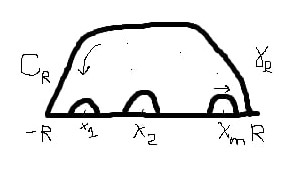
\includegraphics[scale=0.2]{1}
\end{wrapfigure}
Например, возможна и такая картинка.\\
$f_0 \overset{D_{01}}{\equiv} f_1(z)$, а на $\widetilde{D}_{01}$ значения $f_0$ и $f_1$ могут быть различны и тогда $F(z)=f_0(z), \; z \in \widetilde{D}_{01}$, либо $F(z)=f_1(z), \; z \in \widetilde{D}_{01}$

Многозначная (вообще говоря) функция $F(z)$ по построению склеена из однозначных элементов~--- голоморфных функций $f_0, \dotsc, f_n$.

Аналитической функцией $F(z)$ называется набор таких элементов, полученных из исходного элемента $f_0(z)$ аналитическим продолжением по всем цепочкам областей, по которым продолжение возможно.

Эти элементы называют езе голоморфными ветвями. По исходному элементу аналитическая функция строится однозначно.

\subsection{Аналитическое продолжение с помощью степенных рядов}
Одним из алогритмов, реализующих аналитическое продолжение вдоль цепочки областей является аналитическое продолжение с помощью степенных рядов.

Пусть $f_0(z)$ задана в $D_0$ и голоморфна. Возьмём произвольную точку $z_0 \in D_0$ и представим $f_0(z)$ степенным рядом по степеням $z-z_0$.
\[f_0(z) = \sum_{n=0}^\infty c_n(z-z_0)^n\]
Для этого ряда существуют две возможности:
\begin{enumerate}
    \item Радиус сходимости $R_0$ не превосходит расстояния от точки $z_0$ до границы $\partial D_0$ области $D_0$ при любом выборе точки $z_0 \in D_0$.
    Тогда аналитическое продолжение функции $f_0(z)$ из области $D_0$ невозможно.

    \item Существует в области $D_0$ точка такая, что радиус сходимости ряда $R_0 > \rho(z_0, \partial D_0)$. В этом случае область $D_1 = B(z_0, R_0)$ имеет с $D_0$ общую часть $D_{01}$. \\
    \begin{center}
        \begin{tikzpicture}
            \draw (0, 0) circle[radius=1];
            \draw (-2, 0) circle[x radius=2, y radius=0.7];
        
            \begin{scope}
                \clip (0, 0) circle[radius=1];
                \clip (-2, 0) circle[x radius=2, y radius=0.7];    
                \fill[pattern=north east lines] (-2, -2) rectangle(2, 2);
            \end{scope}
            \node[circle, fill, inner sep=0.7pt] at (-0.5, 0) {};
            \node at (-0.5, 0.2) {$z_0$};
            \node at (-2, 0) {$D_0$};
            \node at (0.5, 0) {$D_1$};
            \node at (-1.1, 0.9) {$D_{01}$};
        
        \end{tikzpicture}    
    \end{center}
    В области $D_1$ степенной ряд представляет собой голоморфную функцию $f_1(z)$, которая в $D_{01}$ сопадает с $f_0(z)$ и, следовательно, $f_1(z)$ является непосредственным аналитическим продолжением $f_0(z)$.
    Далее строим таким образом аналитическое продолжение $f_0(z)$ вдоль цепочки кругов.
\end{enumerate}
Вейерштрасс построил пример непродолжаемой функции: $\displaystyle f_0(z) = \sum_{n=0}^\infty z^{2^n}$~--- сходится в круге $B(0,1)$.
На любой дуге $S(0,1)$, даже если она сколь угодно мала, лежит бесконечное число особых точек.

Следует отметить, что продолжение с помощью переразложения степенных рядов малоэффективно. Чаще всего используют другие приёмы.

\subsection{Аналитическое продолжение через границу}
В ряде случаев для аналитического продолжения функции $f_0(z)$, заданной в области $D_0$ используется следующий приём. Пусть области $D_0$ и $D_1$ имеют в качестве общего участка границы кусочно-гладкую кривую $l_{01}$.
Пусть в $D_0$ задана голоморфная функция $f_0(z)$, а в $D_1$~--- голоморфная функция $f_1(z)$, причём $f_0$ непрерывна в $D_0 \cup l_{01}$, а $f_1$ непрерывна в $D_1 \cup l_{01}$ и $f_0 \overset{D_{01}}{\equiv} f_1(z)$.

Тогда $\displaystyle F(z) = 
\begin{cases}
    f_0(z), & z \in D_0 \cup l_{01} \\
    f_1(z), & z \in D_1
\end{cases}$
\quad будет голоморфной в области $D_0 \cup l_{01} \cup D_1$. \\
То есть $f_1$ является непосредственным аналитическим продолжением функции $f_0(z)$ в область $D_1$.

\end{document}